\subsection{Replication}

\subsubsection{Acoustic analysis}
Results from our acoustic analysis can be found in Table \ref{tab:acoustics}. As a reminder, we used \cite{Sulpizio_McQueen_2012}'s original stimuli, but we calculated the acoustic measurements using our own scripts and annotations. We found, like \cite{Sulpizio_McQueen_2012}, that all acoustic measures significantly differed between syllables except for spectral tilt in penultimate words. For antepenultimate words, first syllables were louder (higher amplitude), had a higher pitch (greater f0), were longer in duration, and had greater spectral tilt. For penultimate words, first syllables were louder, had a higher pitch, and were shorter in duration. Thus, while our mean acoustic measurements varied somewhat from those reported in the original \cite{Sulpizio_McQueen_2012}, the overall findings were consistent: amplitude, pitch, duration, and spectral tilt are used productively as acoustic cues to convey lexical stress information and there are clear patterns observed given the stress type. See Figure \ref{fig:raw_acoustics} for detailed comparison across words and syllables. 

\begin{figure}[H]
  \centering
  \includegraphics[width=1\linewidth]{visuals/raw_acoustics_combined.jpeg}
  \caption{The top four plots show individual syllable measurements by stress type with penultimate (black/left facing) and antepenultimate (orange/right facing)  across vowel 1 (left) and vowel 2 (right). Stress competitors are compared using violin plots and line plots between words that have the same base (e.g., \textit{CAlamo} and \textit{caLAta} both have the same base, \textit{cala} ). The lower two line plots show the connections between acoustic cues across an individual word with differences between acoustic measurement scaled and normalized across syllable 1 (middle) and syllable 2 (lower). \hl{Scaling is done by subtracting the group mean from each value and then dividing by the standard deviation. This standardizes the values, centering them around 0 with a spread proportional to the standard deviation.}}
  \label{fig:raw_acoustics}
\end{figure}


\subsubsection{Target and competitor analyses}
Here, we attempt to simplify the modeling approach. \cite{Sulpizio_McQueen_2012} did six separate mixed-effects analyses, three on each stress type corresponding to three additive time windows. \hl{Instead, we use two large models (competitor and target models)} to capture the effects by using stress type as a predictor that could interact with looks over time. \cite{Sulpizio_McQueen_2012}'s method of separating the data into antepenultimate and penultimate data before analysis allows one to examine if looks increase independently in both stress types (antepenultimate and penultimate). However, the separation of these analyses makes it impossible to know if there is a difference between fixations during the process of word recognition for the two stress patterns directly. Said another way, syntagmatic and paradigmatic comparison become possible through combining analyses. \cite{Sulpizio_McQueen_2012} did not find differences in their separate models. In this way, our modeling approach should capture a difference between stress types if there is one. 

Another difference in our analysis is the way that we define time windows of interest. In the original study, there were three time periods for each stress pattern: antepenultimate (200-499 ms, 200-566 ms, 200-669 ms) and penultimate (200-396 ms, 200-566 ms, 200-699 ms). These time windows correspond to the first syllable, first 1.5 syllables, and the second syllable, and allow for a 200 ms delay, which is the estimated time needed to program and launch a saccade \citep{Matin_Shao_Boff_1993}. Like the original study, we have three time windows\hl{; However, due to our combined analyses across syllable,} we used three discrete time windows over the first two syllables of the word that are not additive \hl{to maintain independence for each time windows eye-fixations}: antepenultimate (200-499 ms, 500-566 ms, 567-669 ms) and penultimate (200-396 ms, 397-566 ms, 567-699 ms). That is, we have the first syllable and second syllable as well as a 1.5 window (the average of the first syllable plus half of the second syllable), and the second syllable time window. We did our modeling by starting with a maximal GLM\hl{ER} model defined by predicting binary looks \citep{Barr_2008} in both the target and competitor models. For predictors, we used stress (penultimate-baselines), syllable (syllable 1-baselines) and their interactions. \hl{Finally, we gave participants and words random intercepts and stress random slopes}.

\hl{Model reduction started with a full model including random intercepts, slopes, and their correlations. Correlations were removed first, followed by the slopes, leaving only random intercepts. Models were compared using ANOVA, AIC, and BIC, with convergence checks at each step. Through this process, the following two models provided the best balance of fit, convergence, and simplicity for respective target and competitor analyses:} $$(Target  Fixations \sim Stress * Syllable + (1|Participant)+(1|Word))$$
$$(Competitor  Fixations \sim Stress * Syllable + (Stress|Participant)+(Stress|Word))$$\\
These models had the lowest AIC and BIC values among all models tested, indicating a better fit relative to its complexity. Proportion of looks to targets, competitors, and distractors over the time course of antepenultimate (top) and  penultimate (middle) words can be seen in Figure \ref{fig:raw_pen_vs_anti}. Model outputs can be seen at the bottom of Figure \ref{fig:raw_pen_vs_anti}. \hl{For the Target model, results indicate main effects for syllable. The  1.5 syllable had significantly more looks than the first syllable ($\beta$ = 0.43, \textit{SE} = 0.04, \textit{z} = 10.71, \textit{p} $<$ .001). Similarly, the 2nd syllable had significantly more looks than the first syllable ($\beta$ = 0.46, \textit{SE} = 0.04, \textit{z} = 11.83, \textit{p} $<$ .001). In the competitor model, an effect was only found for the second syllable ($\beta$ = -0.12, \textit{SE} = 0.04, \textit{z} = -3.06, \textit{p} $=$ .002), indicating less looks to competitors during the second syllable.}

\begin{figure}[H]
  \centering
  \includegraphics[width=0.6\linewidth]{visuals/pen_vs_anti_pen_id_combo.jpeg} % Adjust the width as needed
  \caption{Antepenultimate and penultimate fixations over time: The example words CAlamo (antepenultimate) and caLAta (penultimate) are used to show where syllables begin and end by stress type using the vertical dotted lines. Raw data of each participant's proportion of looks to each type of visual stimuli is plotted in thin lines underneath the loess-smoothed proportion of looks across participants. Model output from the target (red) and competitor (blue) analyses can be seen at the bottom of the figure \hl{with standard significance indication of \textless .05, \textless .01, and \textless .001 using *,**, and ***, respectively}}. 
  \label{fig:raw_pen_vs_anti}
\end{figure}

\subsubsection{Target bias analysis}

Following \cite{Sulpizio_McQueen_2012}, we were interested in examining if there was a bias in target looks as a proportion to the total captured fixations across stress types. To do this, we predicted mean looks to targets with stress as a predictor (baseline - antepenultimate). We included \textit{word} and \textit{participant} as random intercepts as well as random slopes for \textit{word} on \textit{participant} intercepts. The most parsimonious model removed random slopes for \textit{word}. Like \cite{Sulpizio_McQueen_2012}'s models, our models found no bias in looks to targets over either stress at any syllable. No significant results were found.   

\subsubsection{Acoustic cue integration}

Finally, we investigated how different acoustic cues influence eye-fixations during word recognition. To do this, we built four mixed-effects models, two for each stress type at syllables 1 and 2, each with identical model structures. For both antepenultimate and penultimate models, target looks were used as the dependent variable with the four scaled measurements of the auditory stimuli (syllable-pitch, syllable-amplitude, syllable-spectral tilt, and syllable-duration). Additionally, \textit{word} and \textit{participant} were given random intercepts. All models started with maximal models and were reduced using a backward stepwise selection procedure. 

\hl{The backward stepwise selection procedure began with the full model, which included all main effects. Non-significant items were removed on the significance levels from Wald z-tests. Each step involved refitting the model without the least significant main effect and comparing the fit of the reduced model to the previous model using AIC. The process continued until the removal of any additional terms resulted in a significant increase in AIC, indicating a poorer fit to the data. This method ensures that the final models were parsimonious, retaining only those predictors that contribute significantly to explaining the variance in target looks.} While \cite{Sulpizio_McQueen_2012} confirmed analyses with reverse regression, their primary analysis focused on correlations between variables and eye-fixations. 

For the antepenultimate syllable 1 model, main effects included spectral tilt ($\beta= 0.18$, \textit{SE} = 0.06, \textit{z} = 2.12, $p = 0.03$), which indicates that target words with higher spectral tilt led to more looks. In the antepenultimate syllable 2 model, main effects of pitch ($\beta= -0.53$, \textit{SE} = 0.22, \textit{z} = -2.4, $p = 0.016$) was found, indicating that higher pitch led to fewer looks to targets. No significant effects were found for either the first or second syllable of the penultimate models. Results can be seen on figure \ref{fig:analysis_3_plot}. \hl{We also did a secondary analysis that includes interactions between speech cues that can be found in our online work\_flow and supplemental materials on OSF, which was designed to allow us to capture more subtle variations across target fixations for Italian word stress. Results can be found on the right side of} figure \ref{fig:analysis_3_plot}. 

\begin{figure}[H]
  \centering
  %\includegraphics[width=1\linewidth]{visuals/analysis_3_plot.jpeg} % Adjust the width as needed
    \includegraphics[width=1\linewidth]{visuals/combined_plot_o_n.jpeg} % Adjust the width as needed

  \caption{Output for antepenultimate and penultimate cue models for first and second syllables. Significance is colorized by model (antepenultimate-orange, penultimate-black). Significance levels 0.05, .01, and .001 are indicated by *,**, and ***, respectively to the right of each syllable. The primary models (left) was described in the text above. The description of the interaction models (right) can be found in the supplementary materials.}
  \label{fig:analysis_3_plot}
\end{figure}

\subsection{Replication summary}
We first corroborated \cite{Sulpizio_McQueen_2012}'s acoustic results using the same stimuli but different methods. Thus, despite increasing researcher degrees of freedom \citep{Corretta2023}, we found the exact same pattern of acoustic differences between the two stress types (see Table \ref{tab:acoustics}).

Next, in our target-competitor analysis, we corroborated \cite{Sulpizio_McQueen_2012}'s findings that looks to the target were greater during the first 1.5 syllables and second syllable across both antepenultimate and penultimate words. Our combined analysis also provided insights into the time course of word recognition across both stress-types: the competitor was disambiguated primarily during the second syllable and looks to targets steadily increased across syllables 1.5 and 2.

Next, we did an analysis of target fixations alone to determine if there was a bias toward looks to penultimate words overall given that the majority of tri-syllabic Italian words have penultimate stress. We once again corroborated \cite{Sulpizio_McQueen_2012}: no bias in looks to targets was found between antepenultimate and penultimate words.

Lastly, we carried out four target analyses involving the four acoustic cues we measured. like \cite{Sulpizio_McQueen_2012} correlation analyses, only antepenultimate acoustic cues were predictive of target fixations. For antepenultimate words during the first syllable, i.e., the stressed syllable, a higher spectral tilt led to more looks to targets. For penultimate words during the first syllable, no acoustic cues were predictive of target fixations.

For antepenultimate words during the second syllable, i.e., the unstressed syllable, a higher pitch led to fewer looks to targets. For penultimate words during the second syllable, i.e., the stressed syllable, again showed no cues to be predictive. 

\subsection{Extension}

Next, we carry out our exploratory individual differences analysis \citep{Yanai2020} using eight behavioral tasks: working memory (measured by digit span), the auditory battery tasks (pitch d$'$, duration d$'$, risetime d$'$, formant d$'$), English and Italian language proficiency (measured by the respective LexTALE or LexITA tasks), and autism spectrum quotient (AQ). The primary aim is to identify which of these measures significantly contribute to target looks during word recognition and how they interact with Italian stress patterns over the first two segmentally identical syllable positions. Centered and regularized individual difference measures can be found in Figure \ref{fig:plot_raw_task}.

\begin{figure}[H]
  \centering
  \includegraphics[width=1\linewidth]{visuals/plot_raw_task.jpeg}
  \caption{Centered data across our eight individual difference behavioral tasks.}
  \label{fig:plot_raw_task}
\end{figure}


For our exploratory analyses, we employed LASSO (Least Absolute Shrinkage and Selection Operator) regression to perform variable selection due to its ability to handle high-dimensional data and multi-collinearity \citep{Zhang2020, Tibshirani1996}. \hl{LASSO works by applying a penalty to the regression coefficients, shrinking some of them towards zero, which effectively excludes less relevant variables from the model. This shrinkage is particularly valuable when dealing with correlated predictors, as it helps in identifying the most important variables while minimizing overfitting.

Early data exploration revealed high correlations between the four battery tasks and moderate correlations between other individual difference measures. LASSO mitigates these issues by penalizing the absolute size of regression coefficients, thereby selecting only the most relevant predictors.

The LASSO model was fit using a $\lambda$ search space, which controls the strength of the penalty. A crucial part of the LASSO procedure is determining the optimal $\lambda$ value that balances model fit and complexity. We used cross-validation to select the best $\lambda$, ensuring that the final model generalizes well to unseen data. Once the significant predictors and their interactions were identified through LASSO, we used these variables to fit a Generalized Linear Mixed Model (GLMM), which provided more detailed insights into how each predictor affects target looks. The GLMM also accounted for random intercepts by word and participant, allowing us to model individual variability effectively.}

\subsubsection{Acoustic cue integration - individual differences}

For all models below, the final models are indicated by the existence of a coefficient in Figure \ref{fig:extened_analysis}. Additional model details are available in our R code. In order to distinguish between individual difference measures and acoustic measures, acoustic measures are called by name alone, while individual difference measures will be called by measure followed by the metric (e.g., acoustic pitch of a word will be called \textit{pitch} and the measure of acoustic sensitivity to pitch will be called \textit{pitch d$'$}) 

The parsimonious antepenultimate syllable 1 model revealed a significant positive effect of pitch d$'$ ($\beta$ = 0.90, \textit{SE} = 0.22, \textit{z} = 4.13, \textit{p} $<$ 0.001) and English LexTALE ($\beta$ = 0.26, \textit{SE} = 0.09, \textit{z} = 2.81, \textit{p} $<$ 0.01), indicating that both better pitch sensitivity and higher English proficiency predict more target fixations. Given that antepenultimate syllables typically have higher duration and amplitude, we interpret the negative interactions in terms of how deviations from these typical acoustic features affect perception. The interaction between duration d$'$ and duration ($\beta$ = -1.00, \textit{SE} = 0.38, \textit{z} = -2.63, \textit{p} $=$ 0.009) and the interaction between risetime d$'$ and spectral tilt ($\beta$ = -0.66, \textit{SE} = 0.27, \textit{z} = -2.45, \textit{p} $=$ 0.01) indicate greater looks to targets for participants with lower duration sensitivity (compared to participants with higher sensitivity) for words with shorter duration. Similarly, for participants with lower risetime sensitivity, greater looks to targets occur for antepenultimate words with lower spectral tilt compared to those with greater sensitivity.

The parsimonious antepenultimate syllable 2 model revealed a negative interaction between pitch and English LexTALE ($\beta$ = -0.44, \textit{SE} = 0.15, \textit{z} = -3.05, \textit{p} $=$ 0.002), indicating that words with higher pitch lead to fewer target fixations by those with higher English proficiency. 

The parsimonious penultimate syllable 1 model was null. No significant predictors or interactions were found.

The parsimonious penultimate syllable 2 model revealed a negative effect of duration d$'$ ($\beta$ = -1.08, \textit{SE} = 0.49, \textit{z} = 2.21, \textit{p} $=$ 0.03) and a positive effect of LexITA ($\beta$ = 0.81, \textit{SE} = 0.20, \textit{z} = 4.11, \textit{p} $<$ 0.001) indicating fewer looks to targets for those with better duration sensitivity and greater looks to targets by participants with greater Italian proficiency scores. Additionally, a positive interaction between formant d$'$ and duration ($\beta$ = 1.17, \textit{SE} = 0.51, \textit{z} = 2.28, \textit{p} $=$ 0.02) was found, indicating higher target looks for words with longer durations by those with better formant discrimination ability. 


%We also evaluated predictors with a k-nearest neighbors (k-NN) model and a random forest model. The decision to use k-nearest neighbors (k-NN) and random forest models in our analysis is grounded in the need to capture complex, non-linear relationships between predictors and outcomes, which might not be fully addressed by parametric methods like LASSO regression. A k-NN with 10-fold cross-validation was applied to predict eye-fixations for each word stress on each syllable using acoustic features and individual difference measures. The optimal number of neighbors was determined to be 5, resulting in an overall accuracy of 72.92\% and a $\kappa$ value of 0.66. The random forest model further identified significant predictors, with syllable-duration having a mean decrease accuracy of 113.73 and a mean decrease gini of 1707.49, syllable-pitch having a mean decrease accuracy of 102.53288 and a mean decrease gini of 1851.24, syllable-spectral tilt having a mean decrease accuracy of 95.065 and a mean decrease gini of 1211.03, and syllable-amplitude having a mean decrease accuracy of 70.23 and a mean decrease gini of 1196.16. Additionally, cognitive measures such as the English Lextale (mean decrease accuracy = 63.10, mean decrease gini = 267.91) and working memory (mean decrease accuracy = 84.98, mean decrease gini = 231.02) were important to the model fit. These findings underscore the importance of integrating both acoustic and cognitive predictors to capture the complexity of word stress perception.

\begin{figure}[H]
  \centering
  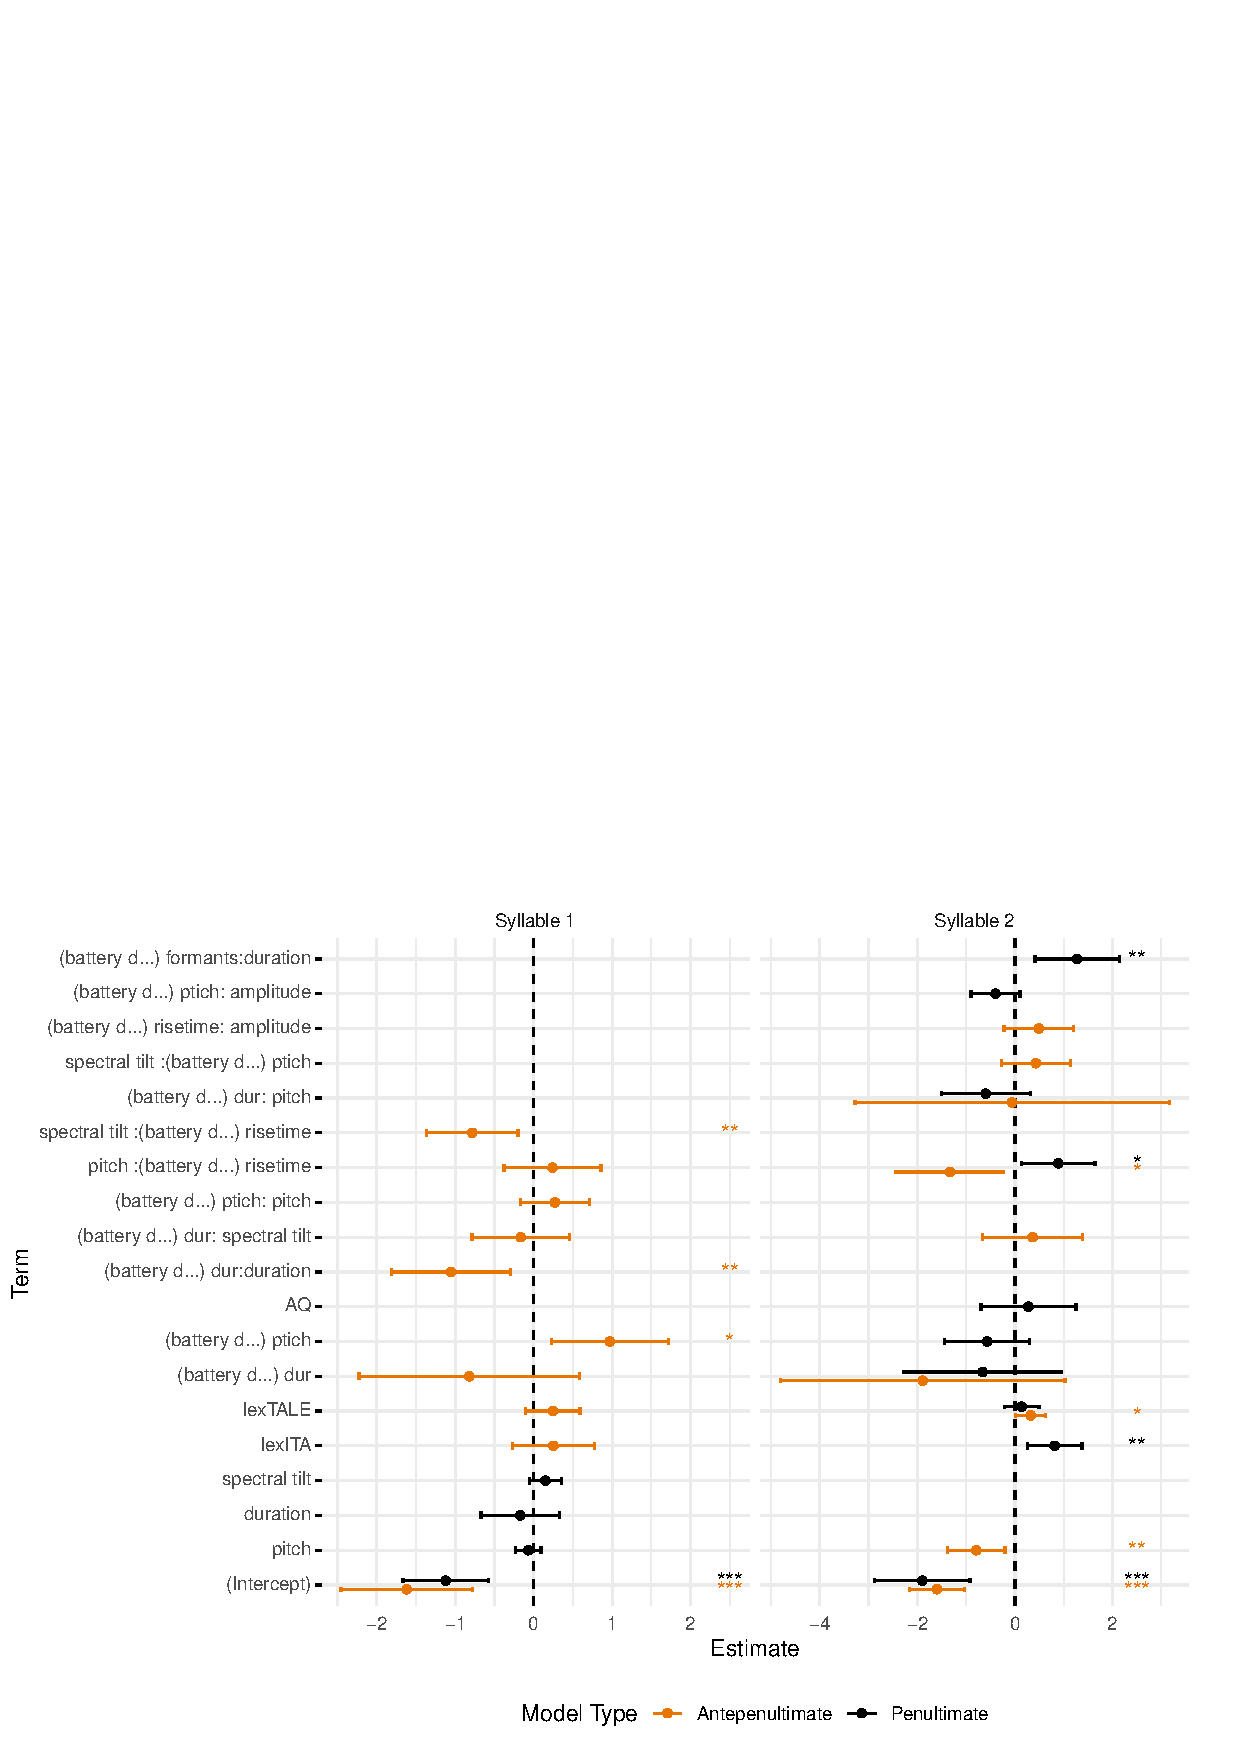
\includegraphics[width=1\linewidth]{visuals/extended_analysis.jpeg} % Adjust the width as needed
  \caption{Antepenultimate and penultimate model output. Significance is colorized by model (penultimate-black, antepenultimate-orange). Significance levels 0.05, .01, and .001 are indicated by standard *,**, and ***, respectively to the right of each syllable.}
  \label{fig:extened_analysis}
\end{figure}


\subsection{Extension summary}

In our exploratory cue integration analysis, for antepenultimate words, participants with higher pitch sensitivity showed more looks to targets during the first syllable. The same pattern was also observed for participants with higher English proficiency. Participants with weaker duration sensitivity showed more looks to targets when the words had shorter durations. Participants with weaker risetime sensitivity also showed more looks to targets when the words had lower spectral tilt. During the second syllable of antepenultimate words, participants with higher English proficiency showed fewer looks to targets with higher pitch. For penultimate words during the first syllable, neither acoustic cues nor individual differences were significant predictors. In the second syllable of penultimate words, participants with higher Italian proficiency showed more looks to targets. Overall, penultimate words with longer second syllable durations had fewer looks, however, participants with greater formant sensitivity showed more looks to targets with longer durations in the second syllable. 